\documentclass{article}
\usepackage[utf8]{inputenc}
\usepackage {indentfirst}
\usepackage{graphicx}

\title{Conversão de Bases}
\author{Introdução a Ciências da Computação}
\date{João Antônio Santos Carvalho - UFSJ}

\begin{document}

\maketitle

 \begin{center}
 \begin{figure}[h]
 \centering
 
\includegraphics[width=8cm]{LOGOUFSJJ.jpg}
 \end{figure}
 \end{center}
 
\section{Objetivo do Trabalho}
O objetivo do trabalho é desenvolver um programa que calcule operações básicas de diferentes bases numéricas, ou seja, soma,subtração,multiplicação e divisão de base binária, octal ou hexadecimal.
\section{Lógica}
\par A lógica pensada para o trabalho foi deixar o usuário selecionar a operação e a base numérica de sua escolha e digitar os números já na base. O programa irá enviar os números para funções auxiliares, as quais irão convertê-los para a base decimal, efetuar o cálculo e convertê-los novamente para a base escolhida, mostrando assim o resultado.
\newpage
\section{Execução do Programa}
\par Ao iniciar o programa irá aparecer um menu e o usuário deve selecionar qual a operação que deseja fazer.
 \begin{center}
 \begin{figure}[h]
 \centering
 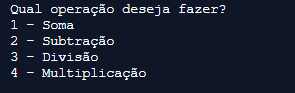
\includegraphics[width=8cm]{menu1.png}
 \end{figure}
 \end{center}
\par Feito isso, aparecerá outro menu, o qual o usuário irá escolher qual base numérica ele fará as operações.
 \begin{center}
 \begin{figure}[h]
 \centering
 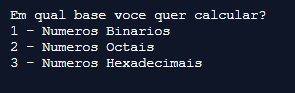
\includegraphics[width=8cm]{menu.png}
 \end{figure}
 \end{center}
 \par Depois de selecionar a operação desejada e a base que irá calcular, deve-se digitar dois números,logo irá aparecer a resposta.
  \begin{center}
 \begin{figure}[h]
 \centering
 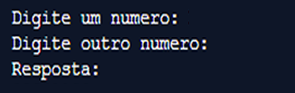
\includegraphics[width=8cm]{numeroeresp.png}
 \end{figure}
 \end{center}
 \newpage
 \section{Programação do Código}
 \subsection{Bibliotecas}
 No começo do código declaramos as bibliotecas, apenas as necessárias. As bibliotecas stdlib.h e stdio.h são as mais comuns, porém inserimos locale.h e string.h, para permitir respectivamente acentuação normal do português na saída de caracteres, e utilização de funções de string.
 \begin{center}
 \begin{figure}[h]
 \centering
 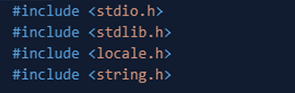
\includegraphics[width=8cm]{bibliotecas.png}
 \end{figure}
 \end{center}
  \subsection{Menu}
  Logo depois, há duas funções para os menus, a primeira para escolher qual operação e a segunda para escolher a base numérica. As duas irão retornar para a função principal as opções escolhidas pelo usuário.
 \begin{center}
 \begin{figure}[h]
 \centering
 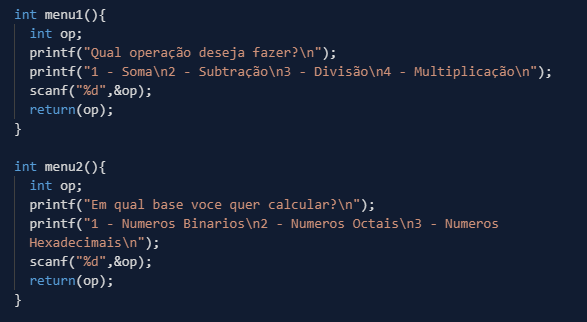
\includegraphics[width=11cm]{fmenu.png}
 \end{figure}
 \end{center}
 \newpage
 
 \subsection{Conversões}
 \subsubsection{Para decimal}
 Segundo a lógica do programa, a função principal irá mandar para as funções auxiliares os números digitados pelo usuário. O programa irá converter tal número da base escolhida para decimal, para efetuar a operação selecionada. 
 \begin{center}
 \begin{figure}[h]
 \centering
 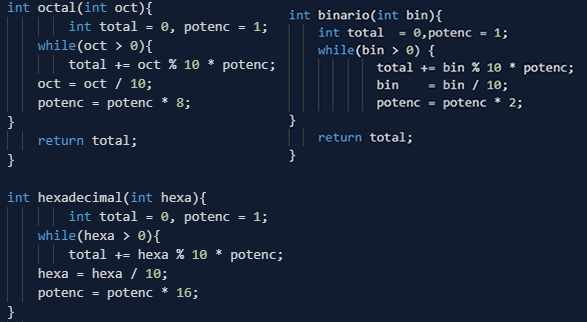
\includegraphics[width=10cm]{func.png}
 \end{figure}
 \end{center}
 \subsubsection{Para a base selecionada}
 Depois de efetuada a operação em decimal, o resultado irá ser convertido para a base escolhida previamente. 
 \begin{center}
 \begin{figure}[h]
 \centering
 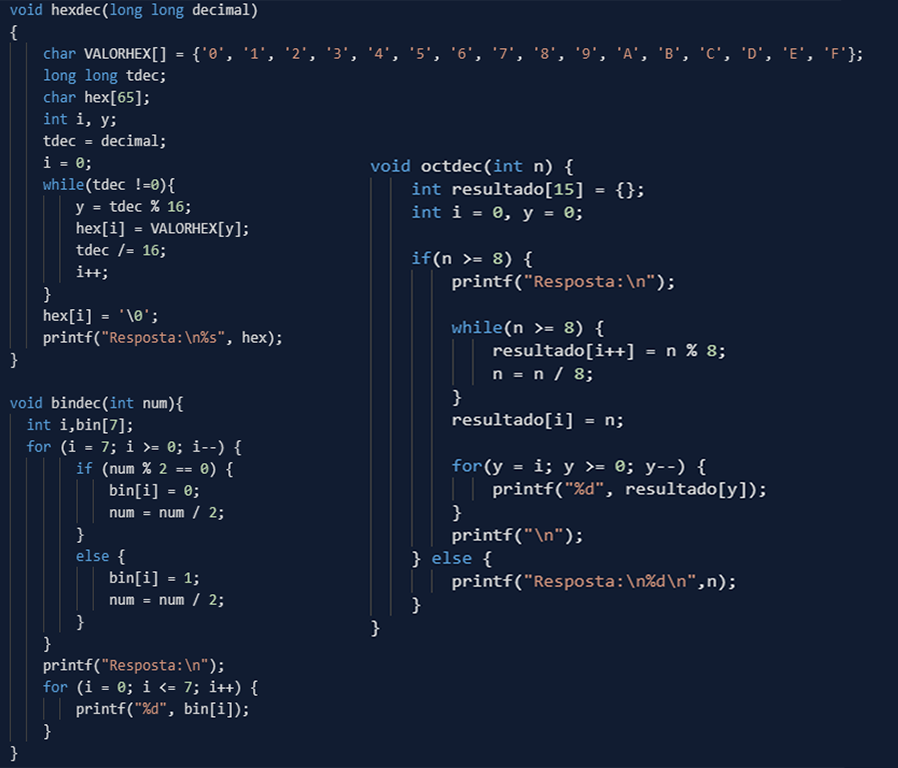
\includegraphics[width=8cm]{func2.png}
 \end{figure}
 \end{center}
 \subsection{Função Principal}
\par Iniciamos a função principal selecionando a língua portuguesa (usando a função locale.h), declaramos as variáveis, sendo que op1 e op2 receberão seus valores das funções dos menus.
 \begin{center}
 \begin{figure}[h]
 \centering
 \includegraphics[width=6cm]{fp.png}
 \end{figure}
 \end{center}
 \par De acordo com esses valores, iniciará os cálculos do programa.
 \begin{center}
 \begin{figure}[h]
 \centering
 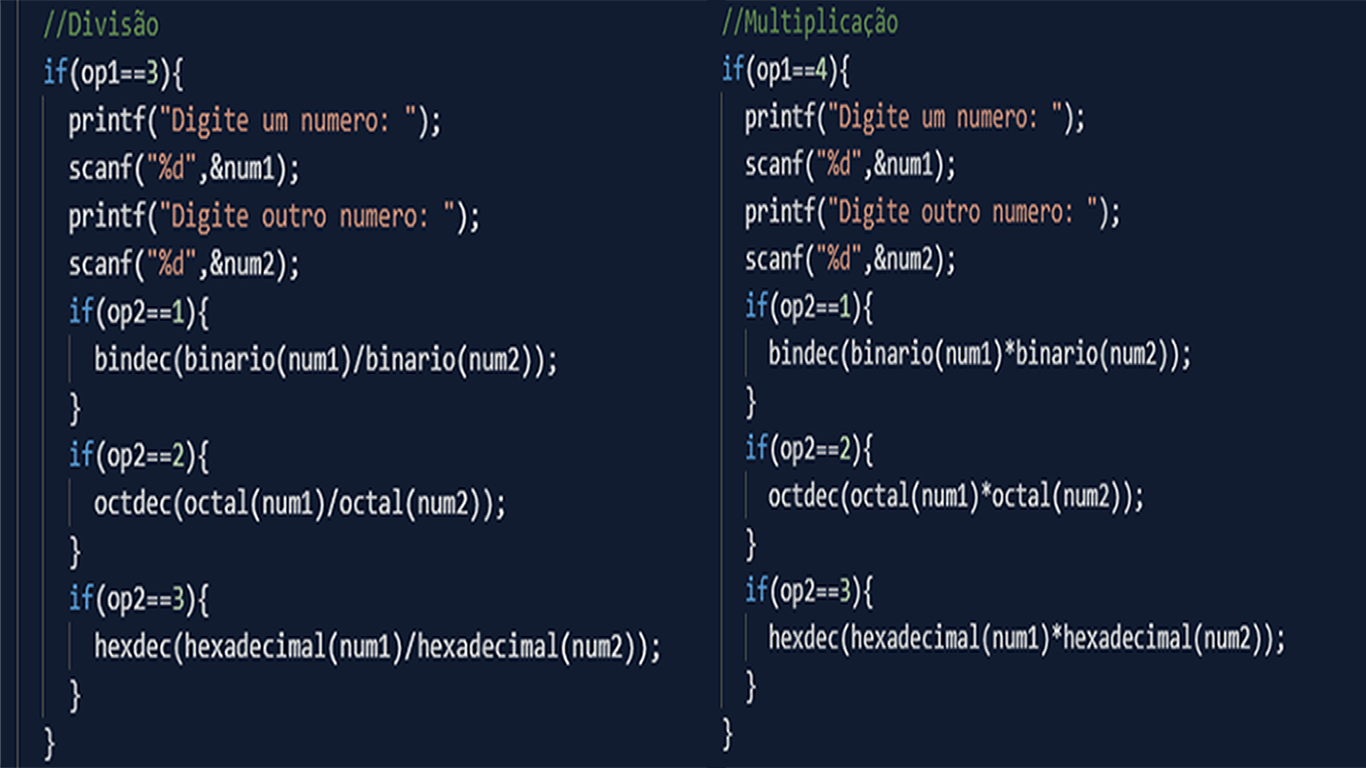
\includegraphics[width=10cm]{dm.png}
 \end{figure}
 \begin{figure}[h]
 \centering
 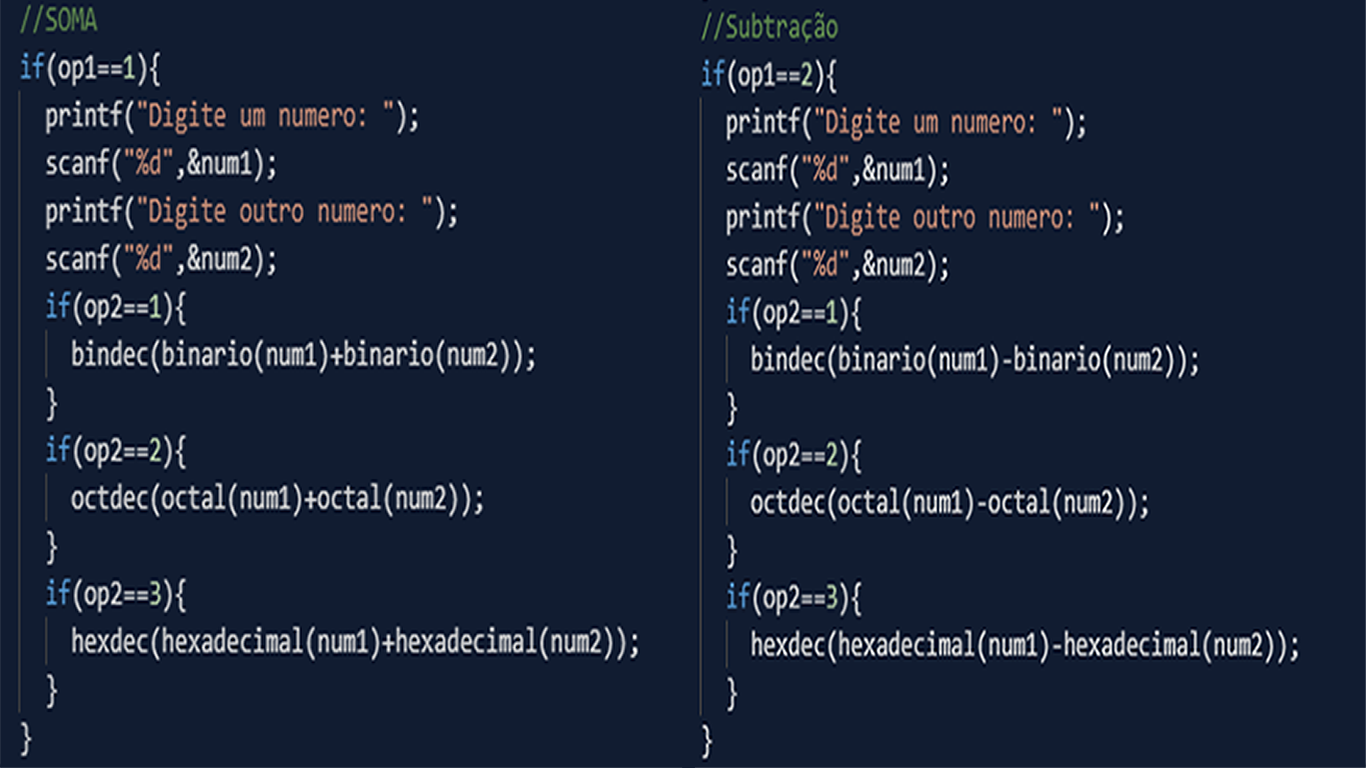
\includegraphics[width=10cm]{ss.png}
 \end{figure}
 \end{center}
 \subsubsection{Excessão}
\par A excessão do código foi as operações adição e subtração de números binários, que foi feito sem conversão.
 \begin{center}
 \begin{figure}[h]
 \centering
 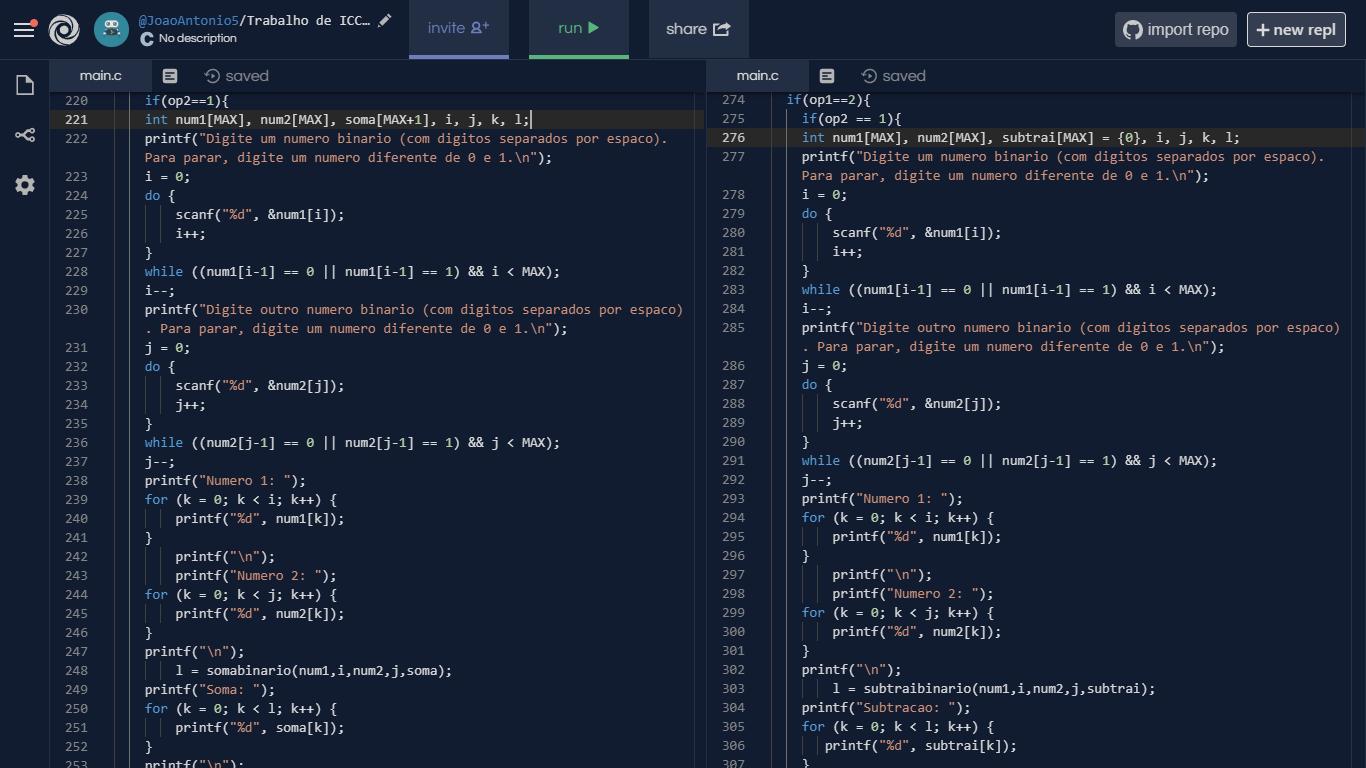
\includegraphics[width=12cm]{exc.png}
 \end{figure}
 \end{center}
\section{Conclusão}
\par Mesmo reunindo várias vezes o grupo não conseguiu resolver o trabalho conforme foi pedido (sem conversão de números), porém o programa funciona do mesmo jeito. Com excessão da soma e subtração de números binários, que com ajuda do monitor conseguimos fazer.
\par Se caso as operações não funcionarem no seu compilador instalado tente em um online, recomendamos esse: https://repl.it/
\end{document}
